\chapter{Marco Teórico}
\section{Conceptos de Visión}

\subsection{Visión Humana}
De una manera muy generar, vision se entiendo como toda accion de ver, sin embargo, desde un punto de vista mas tecnico, vision es la capacidad de interpretar nuestro entorno gracias a los rayos de luz que alcanzan el ojo. Otros autores definen vision como una capacidad necesaria mas no impresindible para realizar las actividades cotidianas.

Desde el punto de la vista de la medicina, la visión humana o sentido de la vista se reduce a un organo receptor conocido como el \textit{ojo}, la membrana y retina son los encargados de recivir las impresiones luminosas para luego transmitirlas al cerebro por medio de las vias opticas(ver figura\ref{fig:estructura_percepcion}). En adicion, el ojo es un organo situado en la cavidad orbitaria, esta protegida por los parpados y por la secrecion de las glandulas lagrumales. 

Los ojos son sensibles a ondas de radiación electromagnética de longitudes específicas. Estas ondas se registran como la sensación de la luz. Cuando la luz penetra en el ojo, pasa a través de la córnea, la pupila y el cristalino, y llega por último a la retina, donde la energía electromagnética de la luz se convierte en impulsos nerviosos que pueden ser utilizados por el cerebro. Los impulsos abandonan el ojo a través del nervio
óptico. La región más sensible del ojo en la visión normal diurna es una pequeña depresión de la retina llamada fóvea en el cual se enfoca la luz que viene del centro del campo visual (por campo visual entendemos aquello a lo que mira el sujeto). Puesto que la lente simple convexa invierte la imagen, el campo visual derecho es representado a la izquierda de la retina y el campo inferior representado en lo alto de la retina. El ojo es un sistema óptico muy imperfecto. Las ondas de luz no solo tienen que pasar a través de los humores y el cristalino, después penetrar la red de los vasos sanguíneos y fibras nerviosas antes de que lleguen las células sensibles los bastones y los conos de la retina donde la luz se convierte en impulsos nerviosos. A pesar de estas imperfecciones el ojo funciona muy bien. La fóvea es capaz de percibir un cable telefónico a 400 m de distancia. En buenas condiciones el ojo puede percibir un alambre cuyo grosor no cubre más de 0,5 mm.

Tambien exister otras definiciones que indican que, el ojo es la puerta de entrada por la que ingresan los estímulos luminosos que se transforman en impulsos eléctricos gracias a unas células especializadas de la retina que son los conos y los bastones. Entonces, el nervio óptico transmite los impulsos eléctricos generados en la retina al cerebro, donde son procesados en la corteza visual. Finalmente, en el cerebro tiene lugar el complicado proceso de la percepción visual gracias al cual somos capaces de percibir la forma de los objetos, identificar distancias, detectar los colores y el movimiento \cite{14alonso2005personas}.


        \begin{figure}[H]
		\centering
		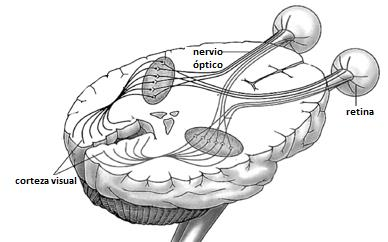
\includegraphics[width=120mm]{./Imagenes/estructura_percepcion.png}
		\caption{Estructura de la percepción visual humana.}
		\vspace{0.15cm}
		\textit{Fuente: Fernando Vila Arroyo, “El Libro Blanco de la Iluminación”. España 2013.}
		\label{fig:estructura_percepcion}
		\end{figure}      	  

\subsection{Visión por Computador}
La visión artificial o también conocida como visión por computador es una disciplina científica que incluye métodos para adquirir, procesar, analizar y comprender las imágenes del mundo real con el fin de producir información numérica o simbólica para que puedan ser tratados por un computador. Tal y como los humanos usamos nuestros ojos y cerebros para comprender el mundo que nos rodea, la visión por computador trata de producir el mismo efecto para que las computadoras puedan percibir y comprender una imagen o secuencia de imágenes y actuar según convenga en una determinada situación. Esta comprensión se consigue gracias a distintos campos como la geometría, la estadística, la física y otras disciplinas. La adquisición de los datos se consigue por varios medios como secuencias de imágenes, vistas desde varias cámaras de video o datos multidimensionales desde un
escáner médico.

Hay muchas tecnologías que utilizan la visión por computador(figura \ref{fig:esquema_vision_computador}), entre las cuáles tenemos: reconocimiento de objetos, detección de eventos, reconstrucción de una escena (\textit{mapping}) y restauración de imágenes \cite{15VC}.


\begin{figure}[H]
		\centering
		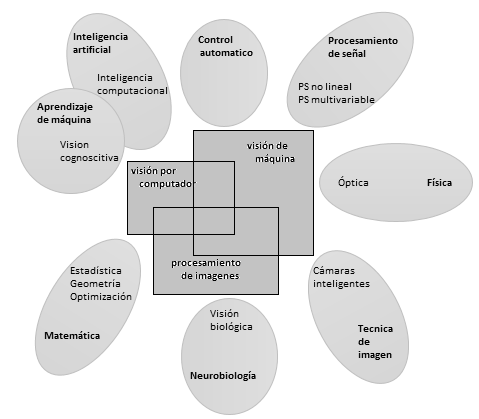
\includegraphics[width=120mm]{./Imagenes/esquema_vision_computador.png}
		\caption{Esquema de las relaciones entre la visión por computadora y otras áreas afines.}
		\vspace{0.15cm}
		\textit{Fuente: Propio}
		\label{fig:esquema_vision_computador}
\end{figure}  


\section{Deteccion de Rostros}
En los últimos años se ha hecho una gran cantidad de esfuerzo en el campo de la detección de rostros. La cara humana contiene características importantes que pueden ser utilizados por los sistemas automatizados basados en la visión con el fin de identificar y reconocer a los individuos. En la localización del rostro, la etapa primaria de los sistemas automatizados basados en la visión es encontrar el área de la cara en la imagen de
entrada. La ubicación exacta de la cara es todavía una tarea difícil. Viola-Jones ha sido ampliamente utilizada por los investigadores con el fin de detectar la ubicación de las caras y los objetos en una imagen dada. Clasificadores de detección de rostros son compartidos por las comunidades públicas, tales como OpenCV \cite{20padilla2012evaluation}.

\subsection{Haar Cascade}
El detector de cara Viola-Jones motivado por el desafío de la detección de rostros, propuso un \textit{framework} detector de objetos utilizando características de tipo \textit{Haar}, que ha sido ampliamente utilizado por otros trabajos, no sólo para la detección de rostros, sino también para la ubicación de objetos. Gracias a la implementación \textit{Open Computer Vision Library}(OpenCV), el framework general de detectores de objetos se ha popularizado y ha motivado a la comunidad a generar sus propios clasificadores de objetos. Estos clasificadores usan características parecidas a las del \textit{Haar} que se aplican sobre la imagen. Solamente aquellas regiones de imagen, llamadas sub-ventanas, que pasan a través de todas las etapas del detector, se considera que contienen el objeto objetivo. La figura \ref{fig:deteccion_cascade} muestra el esquema de cascada de detección con N etapas. La cascada de detección está diseñada para eliminar un gran número de ejemplos negativos con un poco de
procesamiento \cite{20padilla2012evaluation}.

\begin{figure}[H]
		\centering
		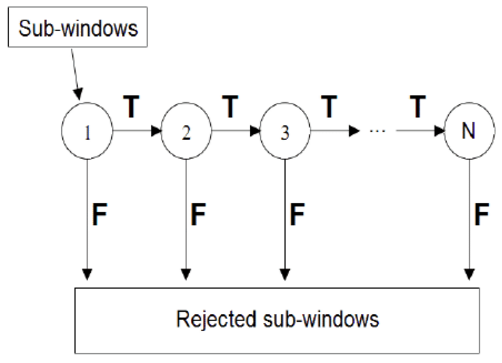
\includegraphics[width=100mm]{./Imagenes/deteccion_cascade.png}
		\caption{Detección Cascade.}
		\vspace{0.15cm}
		\textit{Fuente: Evaluation of Haar Cascade Classifiers for Face Detection.}
		\label{fig:deteccion_cascade}
\end{figure} 

\section{Redes Neuronales}
\subsection{Biológicas}

Son el principal elemento del Sistema Nervioso. Las redes neuronales biológicas son el resultado de la union de varias neuronas entrelazadas entre si. Una neurona es una célula compuesta por tres partes fundamentales: el cuerpo, un numero de extensiones llamadas dendritas que sirven de entradas, y una larga extensión llamada axón, la cual se activa como salida. Existe un proceso de comunicacion entre neuronas, el cual es conocido como 'la sinapsis', este proceso conecta el axón de una neurona a las dendritas de las otras neuronas para comunicarse por medio de impulsos electricos. Las neuronas están dispuestas en multiples capas. Por lo general las neuronas de una primera capa reciben entradas desde otra capa y envían sus salidas o impulsos nerviosos a las neuronas de una tercera. Existe un proceso de retroalimentación que se origina cuando los impulsos nerviosos de una neuronal son enviadas a ella misma, originando asi un ciclo donde la imformacion se mantiene por periodos de tiempo. Similar, puede ocurrir la comunicacion entre neuronas de la misma capa.

Las conexiones entre neuronas tienen pesos asociados que representan la influencia de una sobre la otra. Si dos neuronas no están conectadas, el correspondiente peso de enlace es cero. Esencialmente, cada una envía su información de estado multiplicado por el correspondiente peso a todas las neuronas conectadas con ella. Luego
cada una, a su vez, suma los valores recibidos desde sus dendritas para actualizar sus estados respectivos.

Se emplea normalmente un conjunto de ejemplos representativos de la
transformación deseada para "entrenar" el sistema, que, a su vez, se adapta para producir
las salidas deseadas cuando se lo evalúa con las entradas "aprendidas".

Además, se producirán respuestas cuando, en la utilización, se presenten entradas
totalmente nuevas para sistema, esto es durante el modo entrenamiento la información
sobre el sistema a resolver es almacenada dentro del ANN y la red utiliza su modo
productivo en ejecutar transformaciones y aprender. De este modo el sistema de red
neuronal no reside necesariamente en la elegancia de la solución particular sino en su
generalidad de hallar solución a problemas particulares, habiéndose proporcionado
ejemplos del comportamiento deseado. Esto permite la evolución de los sistemas
autómatas sin una reprogramación explicita.

Las redes neuronales artificiales se basan en el circuito de procesamiento de
entradas en el cual los pesos son sumados. Las funciones de peso serán llamadas desde
ahora como atenuadores. En la implementación, las entradas a una neurona son pesadas
multiplicando el valor de la entrada por un factor que es menor o igual a uno. El valor de
los factores de peso es determinado por el algoritmo de aprendizaje \cite{21RedesNeuronales}.

Las entradas atenuadas son sumadas usando una función no lineal llamada Función
"Sigmoide". Si la salida de la función suma excede el valor de entrada máximo de la
neurona, esta responde generando una salida.

Una persona tiene alrededor de $10^{11}$ neuronas, cada una con alrededor de $10^4$
salidas. La estructura de neuronas de la corteza cerebral es modular: si bien todas las
partes del cerebro son relativamente similares, diferentes partes hacen diferentes cosas; a
partir de una estructura general, según la experiencia se generan nuevas estructuras
especificas al problema a resolver \cite{16pusiol2014redes}. 


\begin{figure}[H]
		\centering
		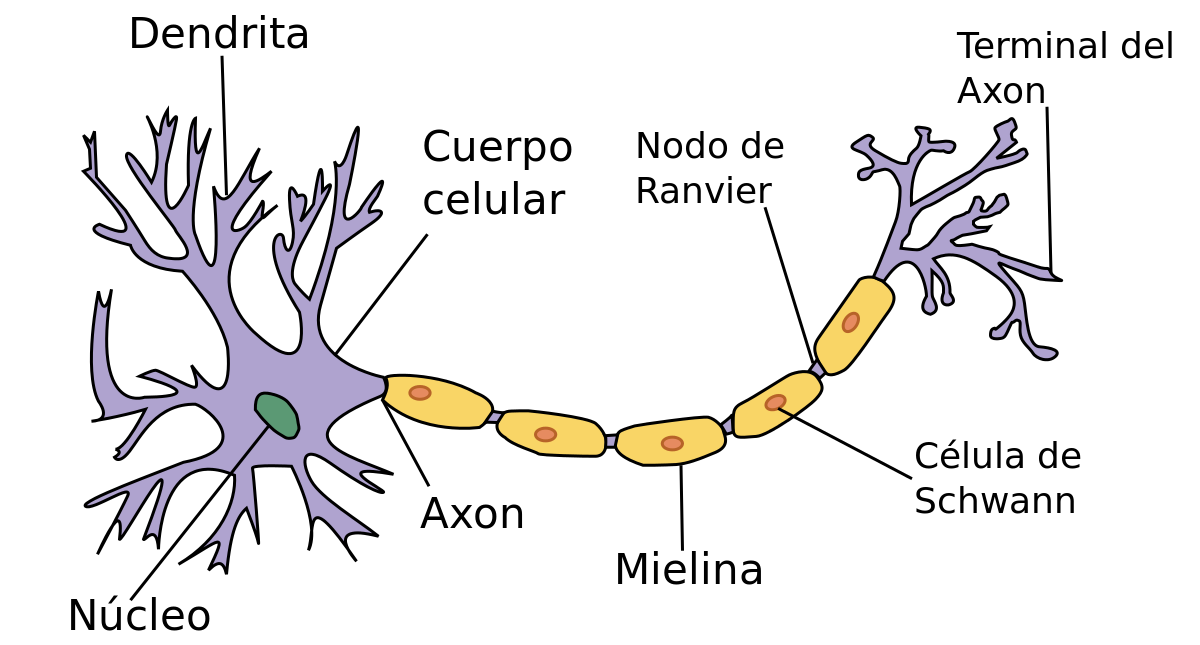
\includegraphics[width=100mm]{./Imagenes/neurona_biologica.png}
		\caption{neuronal biológica}
		Source: Patri Tezanos, Neurociencia, 2016.
		\label{fig:neurona_biologica}
\end{figure} 


\subsection{Artificiales}
Las Redes Neuronales Artificiales (ANN) imitan su funcionamiento a aquellas
que se encuentran en el ámbito biológico. Son aptas para resolver problemas que no
poseen un algoritmo claramente definido para transformar una entrada en una salida;
aprenden, reconocen y aplican relaciones entre objetos.

Se emplea normalmente un conjunto de ejemplos representativos de la
transformación deseada para "entrenar" el sistema, que, a su vez, se adapta para producir
las salidas deseadas cuando se lo evalúa con las entradas "aprendidas".

Además, se producirán respuestas cuando, en la utilización, se presenten entradas
totalmente nuevas para sistema, esto es durante el modo entrenamiento la información
sobre el sistema a resolver es almacenada dentro del ANN y la red utiliza su modo
productivo en ejecutar transformaciones y aprender. De este modo el sistema de red
neuronal no reside necesariamente en la elegancia de la solución particular sino en su
generalidad de hallar solución a problemas particulares, habiéndose proporcionado
ejemplos del comportamiento deseado. Esto permite la evolución de los sistemas
autómatas sin una reprogramación explicita.

Las Redes Neuronales Artificiales se basan en el circuito de procesamiento de
entradas en el cual los pesos son sumados. Las funciones de peso serán llamadas desde
ahora como atenuadores. En la implementación, las entradas a una neurona son pesadas
multiplicando el valor de la entrada por un factor que es menor o igual a uno. El valor de
los factores de peso es determinado por el algoritmo de aprendizaje.

Las entradas atenuadas son sumadas usando una función no lineal llamada
Función "Sigmoide". Si la salida de la función suma excede el valor de entrada máximo
de la neurona, esta responde generando una salida.

Cada neurona tiene varias entradas y su salida está conectada a un conjunto de
otros procesadores de entradas.

Cuando una ANN funciona en modo normal, a partir de los datos presentados en
la entrada, se genera un patrón especifico de salida. La relación Entrada/Salida será
determinada durante el modo entrenamiento, entonces cuando una entrada conocida es
presentada da la salida esperada.

El algoritmo de entrenamiento ajusta los pesos de las entradas hasta que se alcanza
la salida esperada.

Las neuronas en la figura tienen una leve complejidad computacional, porque solo
se comunican con las neuronas más cercanas conectándose de forma simple. Por las
características y capacidades que ofrece la tecnología VLSI es posible (en costos)
construir una Red Neuronal con muchos procesadores \cite{21RedesNeuronales}.


\begin{figure}[H]
		\centering
		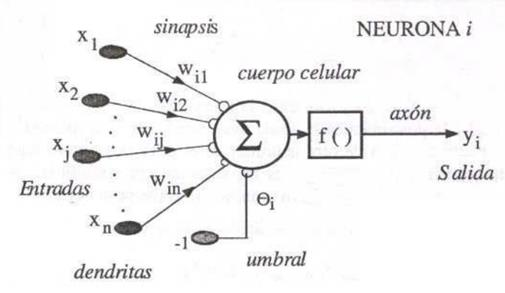
\includegraphics[width=100mm]{./Imagenes/neurona_artificial.png}
		\caption{Modelo matemático de una red neuronal}
		Source: Yuly Cristina Moreira Monserrate, Inteligencia Artificial, 2015.
		\label{fig:neurona_artificial}
\end{figure}

\begin{equation}\label{eq:funcion_salida}
Y_{i} = f(\sum W_{i,j}X{j} - \theta{i})
\end{equation}
Equation \eqref{eq:funcion_salida} Función de salida de una neurona artificial.


\section{ARQUITECTURA DE UNA RED NEURONAL ARTIFICIAL}
\subsection{Capas}

\begin{figure}[H]
		\centering
		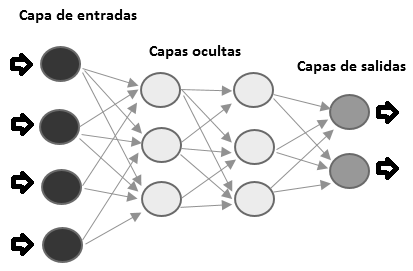
\includegraphics[width=100mm]{./Imagenes/capas_red_neuronal.png}
		\caption{Capas de una red neuronal artificial}
		Source: Propio
		\label{fig:capa_red_neuronal}
\end{figure} 

Una red neuronal se compone de tres capas:
\begin{itemize}
\item \textbf{Capa de Entrada.- }Es la capa que recibe cada uno de los números de la
lista de números entrante correspondientes a la matriz que representa una
imagen.
\item \textbf{Capa Oculta.- }Esta capa contiene unidades no observables, recibe
información de la capa entrante, para posteriormente procesarla y manda
información a la capa de salida.
\item \textbf{Capa de Salida.-} Contiene los resultados como una lista de números.
\end{itemize}


\subsection{Funciones de Activación}
La función de activación recibe como entrada la suma de todos los números que
llegan por las conexiones entrantes, transforma el valor mediante una fórmula, y produce
un nuevo número. Existen varias opciones. Uno de los objetivos de la función de
activación es mantener los números producidos por cada neurona dentro de un rango
razonable (por ejemplo, números reales entre 0 y 1).

\begin{itemize}
\item \textbf{Función de activación Sigmoide}\\

Muchos procesos naturales y curvas de aprendizaje de sistemas complejos
muestran una progresión temporal desde unos niveles bajos al inicio, hasta
acercarse a un clímax transcurrido un cierto tiempo; la transición se produce en
una región caracterizada por una fuerte aceleración intermedia. La función
Sigmoide permite describir esta evolución. Su gráfica tiene una típica forma de
"S". A menudo la función Sigmoide se refiere al caso particular de la función
logística y que viene definida por la siguiente ecuación \cite{24fsigmoide}:

\begin{equation}\label{eq:funcion_sigmoide}
f(x) = \frac{1}{1+\exp^{-x}}
\end{equation}
Equation \eqref{eq:funcion_sigmoide} Función Sigmoide.

\item \textbf{Función de activación Tangencial} \\

Es la versión continua de la función signo y se usa en problemas de
aproximación. Es importante por sus propiedades analíticas. Es continua a valores
en [-1,1] e infinitamente diferenciable, Esta función está definida como \cite{25ftangencial}

\begin{equation}\label{eq:funcion_tanh}
tanh(x) = \frac{\exp^x - \exp^{-x}}{\exp^x + \exp^{-x}}
\end{equation}
Equation \eqref{eq:funcion_tanh} Función Tangencial.


\item \textbf{Función de activación RELU (Rectified Linear Unit)} \\

Se conoce como una función de rampa y es análoga a la rectificación de
onda media en la ingeniería eléctrica. Esta función de activación fue introducida
por primera vez a una red dinámica por Hahnloser et al, en un artículo de año
2000, con fuertes motivaciones biológicas y justificaciones matemáticas. Se ha
utilizado en las Redes Convolucionales con más eficacia que el ampliamente
utilizado Sigmoide logística (que se inspira en la teoría de probabilidades) y su
más práctico contraparte, la tangente hiperbólica . El rectificador es a partir del
2015, la función de activación más popular para las Redes Neuronales Profundas 
\cite{26fRelu}.

\begin{equation}\label{eq:funcion_Relu}
f(x)=Max(0,x)
\end{equation}
Equation \eqref{eq:funcion_Relu} Función RELU.

\end{itemize}
\subsection{Bias o Sesgo}
Justo antes de aplicar la función de activación, cada neurona añade a la suma de
productos un nuevo término constante, llamado habitualmente bias, cuyo único objetivo
es lograr una convergencia más rápida de la red.


\begin{figure}[H]
		\centering
		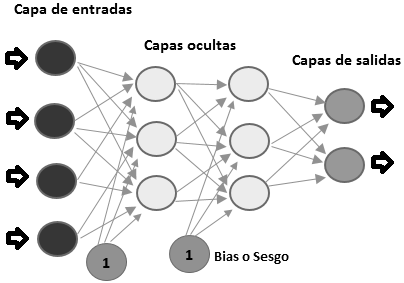
\includegraphics[width=100mm]{./Imagenes/arquitectura_red_neuronal.png}
		\caption{Arquitectura de un RNA incluida el sesgo}
		Source: Propio
		\label{fig:arquitectura_red_neuronal}
\end{figure}

\section{IMPLEMENTACIÓN DE UNA RNA}
Una forma sencilla de implementar redes de neuronas consiste en almacenar los
pesos en matrices. Posteriormente guardar los valores de todas las neuronas de la capa en
un vector, el producto del vector y la matriz de pesos de salida, nos da los valores de
entrada de cada neurona en la siguiente capa. Después se aplica la función de activación
que hayamos elegido a cada elemento de ese segundo vector, y repetir el proceso.

\section{BACKPROPAGATION}
El BackPropagation es un algoritmo de aprendizaje supervisado que se usa para entrenar
redes neuronales artificial, dicho algoritmo se basa en el descenso de gradiente que es un
algoritmo de optimización utilizado para determinar los valores de los parámetros
(coeficientes) de una función (f) que minimiza una función de costes. El descenso de
gradiente se utiliza mejor cuando los parámetros no pueden ser calculados analíticamente
(por ejemplo, usando algebra lineal) y deben ser buscados por un algoritmo de
optimización \cite{27lehr1993backpropagation}.


\begin{figure}[H]
		\centering
		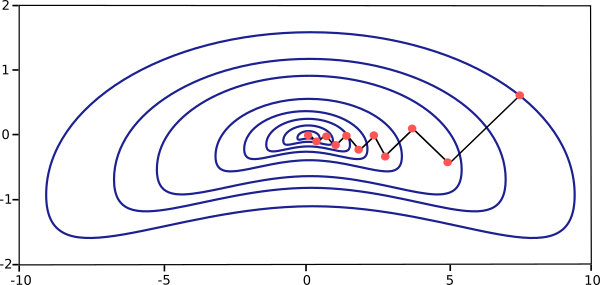
\includegraphics[width=100mm]{./Imagenes/back_propagation.png}
		\caption{Descenso de gradiente}
		Source: Propio
		\label{fig:back_propagation}
\end{figure}


\section{DEEP LEARNING}
El Deep Learning es un concepto muy amplio, lo que conlleva a que no tenga solo
una definición veraz. Sin embargo, se puede generalizar en que el Deep Learning es un
concepto que surge de la idea de imitar el celebro a partir del uso de hardware y software,
para crear una inteligencia artificial pura, utilizando una capacidad de abstracción
jerárquica, es decir, una representación de los datos de entrada en varios “niveles”, en el
caso de las RNA, en varias capas, para seleccionar características que son útiles para el
aprendizaje; de esta manera, una característica de un nivel de complejidad más alto será
aprendido de una de un nivel de complejidad más bajo.

El Deep Learning es un conjunto de algoritmos en Machine Learning que intenta
modelar abstracciones de alto nivel en datos usando arquitecturas compuestas de
transformaciones no-lineales múltiples \cite{17bengio2013representation}.

Dependiendo de la RNA, el algoritmo de entrenamiento de las RNA “más
simples”, de las cuales están compuestas las arquitecturas profundas, se pueden
caracterizar, principalmente, en dos categorías:

\begin{itemize}
\item \textbf{Supervisado: } Se caracteriza porque su entrenamiento es controlado por un agente
externo. Este agente externo “guía” el entrenamiento de la red mediante una
comparación entre las salidas deseadas y las salidas que proporciona la red \cite{18restrepo2015aplicacion}.

\begin{figure}[H]
		\centering
		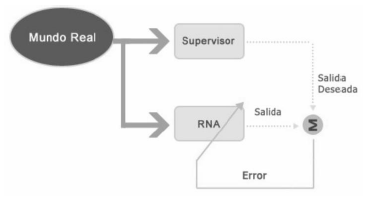
\includegraphics[width=75mm]{./Imagenes/grafico_supervisado.png}
		\caption{Aprendizaje supervisado}
		Source: LÓPEZ S, Jesús A. CAICEDO B, Eduardo F.
		\label{fig:grafico_supervisado}
\end{figure}



\item \textbf{No supervisado: }
El aprendizaje es realizado presentándole a la red los datos
directamente, es decir, ahora no existe un agente supervisando en el
entrenamiento, la red aprende los datos de la entrada modificando los pesos en
función de los datos caracterizados formando, en algunos casos, clusters o
agrupación de los datos, tendiendo a clasificar los datos de forma probabilística
\cite{18restrepo2015aplicacion}.

\begin{figure}[H]
		\centering
		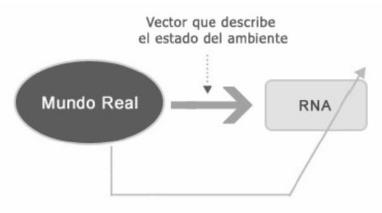
\includegraphics[width=75mm]{./Imagenes/grafico_no_supervisado.png}
		\caption{Aprendizaje no supervisado}
		Source: LÓPEZ S, Jesús A. CAICEDO B, Eduardo F.
		\label{fig:grafico_no_supervisado}
\end{figure}

\item \textbf{Híbrido: }
En las arquitecturas del Deep Learning, algunas redes poseen o utilizan
ambos tipos de entrenamientos, ya sea comenzando con un pre-entrenamiento
supervisado y finalizando con uno no supervisado o viceversa. Esto es con el fin
de lograr un ajuste fino, disminuir el tiempo de convergencia, entre otras
funcionalidades \cite{18restrepo2015aplicacion}.
\end{itemize}
\section{MODELOS MÁS COMUNES DEL DEEP \\LEARNING}
\subsection{Autoencoder}
Es una Red Neuronal Artificial utilizada para el aprendizaje no supervisado
de codificaciones eficientes . El objetivo de una autoencoder es aprender una
representación (codificación) para un conjunto de datos, típicamente con el propósito
de reducción de dimensionalidad . Recientemente, el concepto autoencoder se ha vuelto
más ampliamente utilizado para el aprendizaje de modelos generativos de datos \cite{28fAutoencoder}.

Un auto-codificador, o autoencoder, aprende a producir a la salida exactamente la
misma información que recibe a la entrada. Por eso, las capas de entrada y salida siempre
deben tener el mismo número de neuronas. Por ejemplo, si la capa de entrada recibe los
píxeles de una imagen, esperamos que la red aprenda a producir en su capa de salida
exactamente la misma imagen que ha sido introducido \cite{18restrepo2015aplicacion}.

\begin{figure}[H]
		\centering
		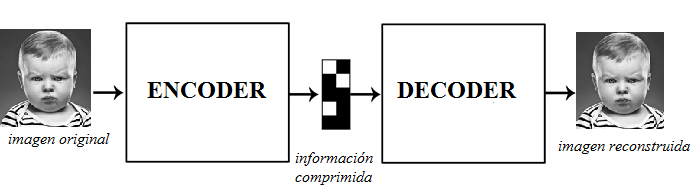
\includegraphics[width=100mm]{./Imagenes/autoenconder.png}
		\caption{Arquitectura de una red neuronal Auto-encoder}
		Source: Propio
		\label{fig:autoencoder}
\end{figure}

\subsection{Redes Neuronales Recurrentes}
Las Redes de Neuronas Recurrentes (Recurrent Neural Networks) no tienen una
estructura de capas, sino que permiten conexiones arbitrarias entre todas las neuronas,
incluso creando ciclos. Esto permite incorporar a la red el concepto de temporalidad, y
permite que la red tenga memoria, porque los números que introducimos en un momento
dado en las neuronas de entrada son transformados, y continúan circulando por la red
incluso después de cambiar los números de entrada por otros diferentes \cite{18restrepo2015aplicacion}.


\begin{figure}[H]
		\centering
		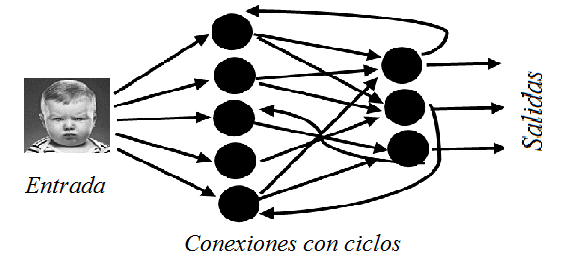
\includegraphics[width=100mm]{./Imagenes/red_recurrente.png}
		\caption{Arquitectura de una red neuronal Recurrente.}
		Source: Propio
		\label{fig:red_recurrente}
\end{figure}

\subsection{Redes Neuronales Convolucionales}
Las Redes Neuronales Convolucionales (Convolution Neural Network) mantienen
el concepto de capas, pero cada neurona de una capa no recibe conexiones entrantes de
todas las neuronas de la capa anterior, sino sólo de algunas. Esto favorece que una neurona
se especialice en una región de la lista de números de la capa anterior, y reduce
drásticamente el número de pesos y de multiplicaciones necesarias. Lo habitual es que
dos neuronas consecutivas de una capa intermedia se especialicen en regiones solapadas
de la capa anterior \cite{16pusiol2014redes}.

\section{ARQUITECTURA DE UNA RED NEURONAL
CONVOLUCIONAL}

Las Redes Neuronales Convolucionales es una estructura compuesta de varias
fases entrenables, aprendiendo de cada una de las características con diferentes grados de
abstracción. La entrada y salida de cada una de estas etapas son conjunto de arreglos
llamados mapas de características, a la salida cada mapa de características representa una
característica particular extraída de la imagen de entrada.

Cada fase está compuesta por tres capas: Convolucion, función no lineal y una
capa de sub-muestreo.

Una típica arquitectura de Red Neuronal Convolucional para clasificación
supervisada está basada en varias etapas seguidas de un clasificador, por ejemplo, la red
de Yann LeCun para resolver el problema de reconocimiento de caracteres, utilizo una
arquitectura con dos fases.


\begin{figure}[H]
		\centering
		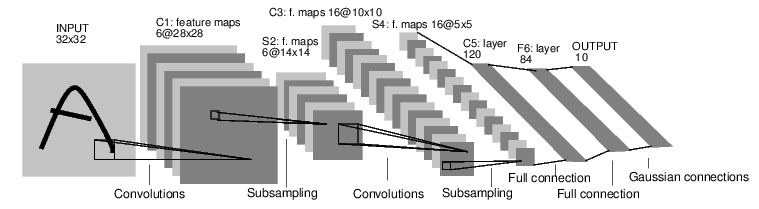
\includegraphics[width=100mm]{./Imagenes/arquitectura_CNN_Lecun.png}
		\caption{Arquitectura de una red neuronal Convolucional.}
		Source: Yann LeCun, 1998.
		\label{fig:arquitectura_CNN_Lecun}
\end{figure}

Viendo el funcionamiento de la arquitectura del Let-Net (Figura 13) toma como
entrada una imagen, y en la entrada de la primera fase hay una secuencia de mapas de
características producto de la convolucion, seguida por una capa de sub-muestreo. En la
capa de convolucion cada uno de los seis mapas de características contiene pequeñas
características con sus pesos agrupados. A continuación, se encuentra la capa del sub-
muestreo que agrupa las salidas de una serie de características replicadas vecinas en la
capa de convolución, dando como resultado un mapa de características más pequeño que
servirá de entrada para la siguiente fase dedicada a encontrar características replicadas de
mayor abstracción. A medida que se avanza en las fases se aprenden características más
complicadas, pero más invariantes a posición (Por el sub-muestreo).

Las capas enteramente conectadas se encargan de evaluar las posibles
combinaciones de las características aprendidas para lograr clasificar las imágenes dadas
\cite{16pusiol2014redes}.

\subsection{Capa de Convolución}
La capa de convolución es el bloque de construcción básico de una red de
convolución que hace la mayor parte del trabajo pesado computacional.
\begin{itemize}
\item \textbf{Visión general e intuición sin cerebro.} La capa de convolución calcula sin
analogías (cerebro / neurona). La capa de parámetros de convolución consisten en
un conjunto de filtros que se pueden aprender. Cada filtro es pequeño
espacialmente (a lo largo de la anchura y altura), sino que se extiende a través de
toda la profundidad del volumen de entrada. Por ejemplo, un filtro típico en una
primera capa de una Red Neuronal Convolucional podría tener un tamaño de
5x5x3 (es decir, 5 píxeles anchura y la altura, y 3 ya que las imágenes tienen
profundidad 3, los canales de color). Durante el pase hacia adelante, se desliza
(más precisamente, convolución) cada filtro a través del ancho y la altura del
volumen de entrada y calcular productos escalares entre las entradas del filtro y la
entrada en cualquier posición. A medida que se desplaza el filtro sobre la anchura
y la altura del volumen de entrada se produce un mapa de activación de 2
dimensiones que da las respuestas de ese filtro en cada posición
espacial. Intuitivamente, la red aprenderá filtros que se activan cuando ven algún
tipo de función visual, como un borde de una orientación o una mancha de un cierto color en la primera capa, o patrones de panal. Después se tendrá todo un
conjunto de filtros en cada capa de convolución (por ejemplo, 12 filtros), y cada
uno de ellos va a producir un mapa de activación de 2 dimensiones por
separado. Vamos a apilar estos mapas de activación a lo largo de la dimensión de
la profundidad y producir el volumen de salida.

\item \textbf{La vista del cerebro.} Cada entrada en el volumen de salida 3D también se puede
interpretar como una salida de una neurona que mira sólo una pequeña región en
los parámetros de entrada y comparte con todas las neuronas a la izquierda y
derecho espacial (ya que todos estos números resultaría de aplicar el mismo
filtro).

\item \textbf{Conectividad local.} Cuando se trata de entradas de alta dimensión como las
imágenes, como se vio anteriormente, no es práctico conectar neuronas a todas las
neuronas en el volumen anterior. En su lugar, se va a conectar cada neurona a sólo
una región local del volumen de entrada. La extensión espacial de esta
conectividad es un hiperparámetro llamado campo receptivo de la neurona
(equivalentemente este es el tamaño del filtro). La extensión de la conectividad a
lo largo del eje de profundidad es siempre igual a la profundidad del volumen de
entrada. Es importante destacar nuevamente esta asimetría en cómo tratamos las
dimensiones espaciales (anchura y altura) y la dimensión de la profundidad: Las
conexiones son locales en el espacio (a lo largo del ancho y la altura), pero siempre
llenas a lo largo de toda la profundidad del volumen de entrada \cite{22RedesNeuronalesConvolu}.


\begin{figure}[H]
		\centering
		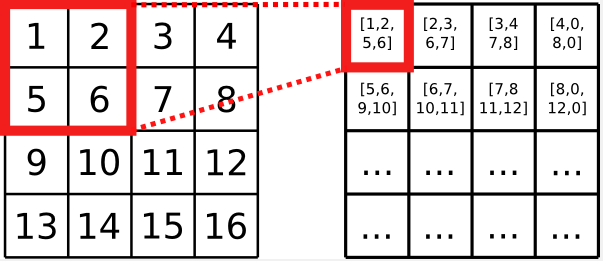
\includegraphics[width=70mm]{./Imagenes/convolucion.png}
		\caption{Ejemplo de convolución con una ventana de 2X2}
		Source: Rubén López, https://rubenlopezg.wordpress.com/2014/05/07/que-es-y-como-funciona-
deep-learning/
        \label{fig:convolucion}
\end{figure}


\item { \textbf{Pseudo – Codigo.} Los valores de un píxel dado en la imagen de salida se calculan
multiplicando cada valor del kernel por los valores de píxeles de la imagen de
entrada correspondientes. Esto se puede describir algorítmicamente con el
siguiente pseudo-código:

%\vspace{6cm}

\begin{algorithm}
\caption{Pseudo-Codigo Convolucion\\
La convolucion de una image f(x,y) con un kernel k(x,y) con dimensiones HxW y (2h+1)x(2w+1) respectivamente produce una nueva imagen g(x,y)}\label{alg:euclid}
\begin{algorithmic}[H]
\Procedure{Convolucion}{$f,k$}\Comment{La convolucion de la imagen f con el kernel k}

\For{\texttt{y:=1 to W}}

\For{\texttt{x:=1 to H}}
  \State $sum=0$
     \For{\texttt{i:=-h to h}}
		\For{\texttt{j:=-w to w}}
           \State $sum=sum + k(j,i)*f(x-j,y-i)$
		\EndFor
	 \EndFor 
  \State $g(x,y)=sum$
\EndFor
\EndFor
\State \textbf{return} $g$\Comment{El resultado de la convolucion entre f y k}
\EndProcedure
\end{algorithmic}
\end{algorithm}


\begin{equation}\label{eq:ecuac_conv}
V = \frac{\sum^{q1}_{i=0}\sum^{q2}_{i=j} f_{i,j}*k_{i,j}}{F}
\end{equation}
Equation \eqref{eq:ecuac_conv} Formula de Convolución.
\\
Donde:\\
\begin{itemize}
\item $f_{i,j}$: El pixel en la posición $i,j$ de la imagen f respecto al kernel k.
\item $k_{i,j}$: El pixel en la posición $i,j$ del kernel k.
\item $q1xq2 = (2h+1)x(2w+1)$: La dimension del kernel.
\item F: La suma de los coeficientes del kernel, o 1 si la suma es igual a 0.
\item g(i,j): El valor de salida de un pixel.
\end{itemize}}

\end{itemize}


\subsection{Submuestreo}
Es común insertar periódicamente una capa de agrupación entre capas sucesivas
de convolución en una arquitectura de Red Neuronal Convolucional. Su función es
reducir progresivamente el tamaño espacial de la representación para reducir la cantidad
de parámetros y el cálculo en la red, y por lo tanto también para controlar el sobre ajuste.
La capa de agrupación funciona independientemente en cada segmento de profundidad
de la entrada y la redimensiona espacialmente, utilizando la operación MAX. La forma
más común es una capa de agrupación con filtros de tamaño 2x2 aplicado con una zancada
de 2 muestras descendentes cada porción de profundidad en la entrada por 2 a lo largo
tanto de ancho como de altura, descartando el 75\% de las activaciones. En este caso, cada
operación MAX tomaría un máximo de 4 números (pequeña región 2x2 en una parte de
profundidad). La dimensión de profundidad no cambia. Más generalmente, la capa de
agrupación:

\begin{itemize}
\item Acepta un volumen de tamaño W1xH1xD1
\item Requiere 2 hiperparámetro
  \begin{itemize}
  \item Su extensión espacial F
  \item La zancada S
  \end{itemize}
\item Produce un volumen de tamaño: W2xH2xD2
  \begin{itemize}
  \item $W2 =  \frac{W1 - F}{S + 1}$
  \item $H2 = \frac{H1 - F}{S + 1}$
  
  \item D2 = D1
  \end{itemize}
\item Introduce parámetros cero, ya que calcula una función fija de la entrada.
\item Tiene en cuenta que no es común utilizar cero como relleno para las capas de
agrupación
\end{itemize}

Sólo hay dos variaciones comunes de la capa de agrupación máxima encontrada
en la práctica: Una capa de agrupación con F = 3, S = 2F, S = 2 (también llamada
superposición de agrupación) y más comúnmente F = 2, S = 2F, S = 2 Los tamaños
de agrupación con campos receptivos más grandes son demasiado destructivos \cite{22RedesNeuronalesConvolu}.

\begin{figure}[H]
		\centering
		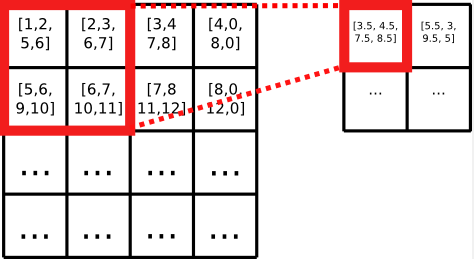
\includegraphics[width=100mm]{./Imagenes/submuestre.png}
		\caption{Ejemplo de Submuestreo con una ventana de 2X2 y calculando el promedio}
		Source: Rubén López, https://rubenlopezg.wordpress.com/2014/05/07/que-es-y-como-funciona-
deep-learning/
        \label{fig:submuestre}
\end{figure}


\subsection{Capa de normalización}
Normalizar las activaciones de la capa anterior en cada lote, es decir, se aplica una
transformación que mantiene la activación de cierre media de 0 y la desviación estándar
de activación cerca de 1 \cite{22RedesNeuronalesConvolu}.

\subsection{Capa totalmente conectada}
Las neuronas en una capa completamente conectada tienen conexiones completas con
todas las activaciones en la capa anterior, como se ve en las redes neuronales regulares.
Por tanto, sus activaciones pueden calcularse con una multiplicación matricial seguida de
un desplazamiento de polarización \cite{22RedesNeuronalesConvolu}.


\begin{figure}[H]
		\centering
		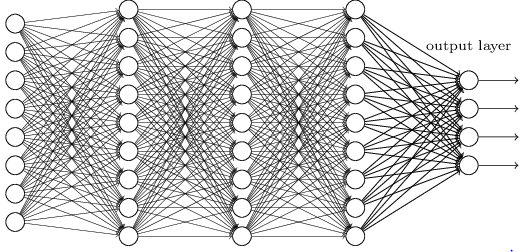
\includegraphics[width=100mm]{./Imagenes/grafico_full_conect.png}
		\caption{Capa totalmente conectada}
		Source: Michael A. Nielsen, http://neuralnetworksanddeeplearning.com/chap6.html
		\label{fig:grafico_full_conect}
\end{figure}

\subsection{Función de normalización(Softmax)}
La regresión softmax es sólo otro nombre para regresión lineal multinomial o
simplemente clase múltiple de regresión logística.

En su esencia, regresión de softmax es una generalización de la regresión logística
que podemos utilizar para la clasificación de clase múltiple (bajo el supuesto de que las
clases son mutuamente excluyentes). En cambio, utilizamos el modelo de regresión
logística (estándar) en tareas de clasificación binario.

\begin{figure}[H]
		\centering
		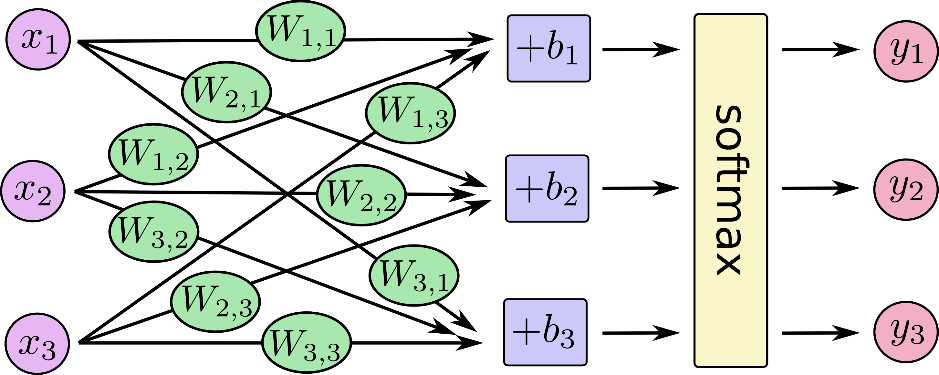
\includegraphics[width=100mm]{./Imagenes/arquitectura_cnn_softmax.png}
		\caption{Arquitectura de una CNN con Softmax}
		Source: Samuel Salvatella, http://ssalva.bitballoon.com/blog/2016-08-30-tensorflow/
		\label{fig:arquitectura_cnn_softmax}
\end{figure}


En las matemáticas , la función softmax , o función exponencial normalizada , es
una generalización de la función logística que permite la utilización de un vector de
dimensión.. La función está dada por

\begin{equation}\label{eq:ecuac_soft}
P(Y = j|Z^i) = \phi_{softmax}(Z^i)= \frac{\exp^{Z^i}}{\sum^k_{j=0}\exp^{Z^{i}_k}}
\end{equation}
Equation \eqref{eq:ecuac_soft} Formula softmax, Donde:\\
$Z = w_{0}x_{0} + w_{1}x_{1} +...+w_{m}x_{m} = \sum_{l=0}^m w_{l}x_{l} = w^Tx$


\section{ENTRENAMIENTO DE UNA RED NEURONAL CONVOLUCIONAL}

El proceso de la CNN para la parte del entrenamiento utiliza el algoritmo
BackPropagation que consiste en calcular una función objetivo que es el de minimizar el
error haciendo para esto la retro propagación del error obtenido a las capas anteriores a la
salida para que se ajusten los pesos de las conexiones entre neuronas.

El algoritmo BackPropagation trabaja de la siguiente forma:

\begin{itemize}
\item Se dan datos de entrada a la red neuronal.
\item Propaga dichas entradas hasta la capa de salida con pesos iniciales definidos o
aleatorios.
\item Calcula el error en la capa de salida.
\item Propaga dicho error hacia las neuronas ocultas (hacia atrás).
\item Cambia los pesos de las conexiones.
\end{itemize}

\section{SOBRE LAS EXPRESIONES FACIALES}
\subsection{Paul Ekman}

Después de que su madre desarrolló una enfermedad mental y se suicidó, Paul
Ekman (psicólogo y científico del comportamiento) dedicó su vida a la Psicoterapia y
ayudar a las personas con trastornos mentales. Él comenzó su investigación en la
comunicación no verbal en la década de 1950, el desarrollo de maneras sistemáticas para
medir el lenguaje corporal. En el proceso, descubrió que, a través de la investigación
empírica, pudo identificar constantemente las expresiones faciales creadas por el
movimiento de los músculos de la cara. Y así, Ekman amplió su investigación para incluir
expresiones faciales y sus significados\cite{29ekman2016scientists}.


\subsection{Las seis emociones básicas}
Antes de Ekman llegó a la escena, se creía ampliamente (por antropólogos
incluyendo Margaret Mead) que las expresiones faciales y las emociones que ellos
representan se determinaron por la cultura – que las personas aprendieron a hacer y leer
las expresiones faciales de sus sociedades. Ekman se dispuso a probar esta idea en
1968. Él viajó a Papúa Nueva Guinea para estudiar las expresiones faciales de los
miembros de la tribu Fore apartada, donde aprendió que podían identificar
constantemente las emociones en las expresiones faciales por mirar fotos de la gente de
otras culturas, a pesar de que la tribu no había sido expuesta a cualquier exterior culturas.

Se hizo evidente, entonces, que las expresiones faciales son interculturales, su
investigación reveló que existe un conjunto universal de ciertas expresiones faciales se
utilizan tanto en el mundo occidental y oriental. Esta lista de expresiones faciales
universales, que Ekman publicó en el año 1972, dispone de las seis emociones
básicas. Tomar por lo vistazo a la lista, así como imágenes, definiciones y movimientos
musculares de estas emociones, a continuación:

\begin{itemize}
\item {\textbf{Cólera:} 
\begin{itemize}
\item \textbf{Descripción.-} El antagonismo hacia una persona o un objeto a menudo se sentía
después de que usted siente que ha sido agraviado u ofendido.
\item { \textbf{Movimientos musculares faciales.-} La reducción de las cejas, apretar y estrechar
los labios, los ojos mirando, apretando los párpados inferiores, con menos
frecuencia, empujando la mandíbula hacia adelante.

\begin{figure}[H]
		\centering
		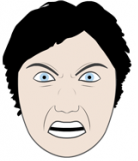
\includegraphics[width=20mm]{./Imagenes/colera.png}
		\caption{Expresión Facial de Cólera}
		Source: Paul Ekman, http://www.serperuano.com/2014/03/paul-ekman-las-6-emociones-basicas/
		\label{fig:colera}
\end{figure}}
\end{itemize}}



\item {\textbf{Felicidad:} 
\begin{itemize}
\item \textbf{Descripción.-} Agradable sensación de satisfacción y bienestar.
\item { \textbf{Movimientos musculares faciales.-} Smiling – tirando hacia arriba comisuras de
la boca, contrayendo los músculos grandes orbitales alrededor de los ojos.

\begin{figure}[H]
		\centering
		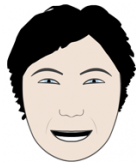
\includegraphics[width=20mm]{./Imagenes/felicidad.png}
		\caption{Expresión Facial de Felicidad}
		Source: Paul Ekman, http://www.serperuano.com/2014/03/paul-ekman-las-6-emociones-basicas/
		\label{fig:felicidad}
\end{figure}}
\end{itemize}}



\item {\textbf{Sorpresa:} 
\begin{itemize}
\item \textbf{Descripción.-} Sensación de malestar o sorpresa ante un hecho inesperado.
\item { \textbf{Movimientos musculares faciales.-} Levantando las cejas altas (que puede causar
arrugas en la frente), abriendo los ojos como platos, dejando caer la mandíbula
tan boca es ágape.

\begin{figure}[H]
		\centering
		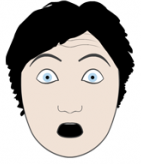
\includegraphics[width=20mm]{./Imagenes/sorpresa.png}
		\caption{Expresión Facial de Sorpresa}
		Source: Paul Ekman, http://www.serperuano.com/2014/03/paul-ekman-las-6-emociones-basicas/
		\label{fig:sorpresa}
\end{figure}}
\end{itemize}}


\item {\textbf{Asco:} 
\begin{itemize}
\item \textbf{Descripción.-} Desagrado intenso o condena causada por algo ofensivo o
repulsiva.
\item { \textbf{Movimientos musculares faciales.-} La reducción de las cejas, curvando el labio
superior, arrugando la nariz.

\begin{figure}[H]
		\centering
		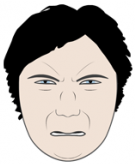
\includegraphics[width=20mm]{./Imagenes/asco.png}
		\caption{Expresión Facial de Asco}
		Source: Paul Ekman, http://www.serperuano.com/2014/03/paul-ekman-las-6-emociones-basicas/
		\label{fig:asco}
\end{figure}}
\end{itemize}}



\item {\textbf{Tristeza:} 
\begin{itemize}
\item \textbf{Descripción.-} Sentimiento de infelicidad o tristeza.
\item { \textbf{Movimientos musculares faciales.-} Los párpados caídos, la reducción de las
esquinas de la boca, labios fruncidos, los ojos bajos.

\begin{figure}[H]
		\centering
		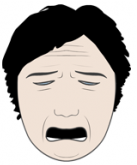
\includegraphics[width=20mm]{./Imagenes/tristeza.png}
		\caption{Expresión Facial de Tristeza}
		Source: Paul Ekman, http://www.serperuano.com/2014/03/paul-ekman-las-6-emociones-basicas/
		\label{fig:tristeza}
\end{figure}}
\end{itemize}}


\item {\textbf{Miedo:} 
\begin{itemize}
\item \textbf{Descripción.-} Sensación de aprehensión provocada por la percepción de peligro,
amenaza o imposición de dolor.
\item { \textbf{Movimientos musculares faciales.-} Levantando las cejas / dibujar las cejas
juntas, tensando los párpados inferiores, que se extiende horizontalmente labios,
la boca ligeramente abierta.

\begin{figure}[H]
		\centering
		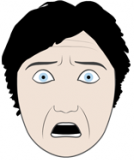
\includegraphics[width=20mm]{./Imagenes/miedo.png}
		\caption{Expresión Facial de Miedo}
		Source: Paul Ekman, http://www.serperuano.com/2014/03/paul-ekman-las-6-emociones-basicas/
		\label{fig:miedo}
\end{figure}}
\end{itemize}}

\end{itemize}


\subsection{Otras expresiones faciales}
Los hallazgos de Ekman sobre las expresiones faciales universales revelaron el
carácter intercultural de la relación entre la comunicación no verbal y la emoción, sin
embargo, las teorías de Ekman han evolucionado desde que ideó su lista de emociones
básicas. En la década de 1990, añadió una serie de otros a la lista de emociones
universales, aunque hizo hincapié en que no todos ellos pueden ser identificados
utilizando expresiones faciales. Estas emociones adicionales son \cite{29ekman2016scientists}

\begin{itemize}
\item Diversión
\item Desprecio
\item Contentamiento
\item Vergüenza	
\item Emoción
\item Culpa
\item El orgullo de los logros
\item Alivio
\item Satisfacción
\item Placer sensorial
\item Vergüenza
\item Neutro
\end{itemize}
